\documentclass[11pt,a4paper]{ctexart}
\usepackage[a4paper,margin=2.2cm]{geometry}
\usepackage{amsmath,amssymb,mathtools,bm}
\usepackage{booktabs}
\usepackage{graphicx}
\usepackage{float}
\usepackage{enumitem}
\usepackage{hyperref}
\usepackage{siunitx}
\usepackage{xcolor}
\usepackage{microtype}
\usepackage{threeparttable}
\usepackage{longtable}
\usepackage{placeins}
\hypersetup{colorlinks=true,linkcolor=blue!60!black,urlcolor=blue!60!black,citecolor=blue!60!black}
\setlist[itemize]{leftmargin=2em,itemsep=0.2em,topsep=0.2em}
\setlist[enumerate]{leftmargin=2.2em,itemsep=0.2em,topsep=0.2em}
\setlength{\parskip}{0.35em}
\setlength{\parindent}{2em}
\graphicspath{{results/figures/}}
\title{基于 SDF 原生窄带累加的通用压力场接触动力学框架\\Sprint 3 附录扩展版}
\author{}
\date{2026年4月}

\begin{document}
\maketitle

\begin{abstract}
本文面向一种通用的 SDF-native 压力场接触（PFC）动力学框架，给出 Sprint 1 阶段的完整投稿闭环。与将显式接触面恢复作为默认求解路径的实现不同，本文保留对象固定压力场与等压平衡的物理闭包，同时将默认数值主链改写为基于 signed distance function (SDF) 的窄带/稀疏 active-cell 累加：几何由 SDF 表示，局部压力由深度场驱动，平衡条件由压力差场 $h=p_A-p_B$ 给出，合力与合力矩直接在窄带 active cells 上累计，而不再把 sheet/mesh 重建作为每一步动力学求解的前置条件。围绕这条主链，当前代码进一步实现了 continuity-aware warm start、boundary-only update、predictor/corrector continuity controller、event-aware midpoint、impulse-corrected accepted step、work-consistent accepted step 以及 per-cell consistent traction reconstruction。

本文的 Sprint 1 贡献不再停留在单个 benchmark 或散乱脚本层面，而是形成了可复现、可导表、可导图的实验基础设施。项目现在包含统一的配置文件、主表脚本、效率表脚本、图生成脚本和导表工具，能够一键生成长时程 flat/sphere/native-band 主表、效率表以及论文主图。现有结果支持以下阶段性结论：第一，SDF-native 主链已经完整打通；第二，continuity-aware traversal 在不明显带偏主结果的前提下显著降低了 traversal 成本；第三，时间一致性的两轮改进链（impulse correction 与 work consistency）在长时程 flat/sphere benchmark 中系统改善了冲量、能量与释放阶段的动力学指标。与此同时，本文也保持审慎：当前 strongest evidence 仍集中在 analytic flat、analytic sphere 与 native-band flat 三组基准上，更一般三维复杂动态接触上的长时程证据链仍需继续补强。
\end{abstract}

\tableofcontents

\section{引言}
接触动力学中始终存在一个张力：高精度几何与力学闭包往往要求复杂的接触面恢复、patch 拓扑维护和高成本 surface quadrature，而高效时间推进又要求每一步的接触求值足够局部、足够稀疏、足够稳定。这个矛盾在 flat large-area contact 中尤为突出：静力与准静力通常可以做得很好，但一旦进入动力学，first-contact、active-region 激活、冲量累计和能量一致性都会放大离散误差。

本文采取的策略不是重新发明一套显式曲面接触算法，而是保留 PFC 的物理主干，将默认数值求解器改造成 \textbf{SDF-native} 的窄带累加器。我们把 marching-cubes、curved-sheet reconstruction 等显式表面重建技术降格为参考链与调试链，而把真正的动力学主链建立在 SDF 所定义的体场之上：由深度场构造压力场，再由压力差场构造平衡条件，最后在窄带 sparse active cells 上直接累计 wrench。围绕这条主链，Sprint 1 的重点不是继续堆新算法，而是完成一套投稿闭环：统一实验入口、统一配置、统一导表导图、并将长时程 flat/sphere/native-band 结果组织成一条清晰的 ablation 故事。

\noindent\textit{For all native-band experiments in this paper, native-band now uses cell-centered volumetric sampling and cell-centered footprint support masking.}

本文的主要贡献概括为三点：
\begin{enumerate}
    \item 提出并实现了一种 \textbf{SDF-native 的 PFC 动力学求解主链}，以窄带/稀疏 active-cell 累加取代显式接触面恢复作为默认路径。
    \item 构造了一条 \textbf{无几何特调的通用动态一致性机制}，包括 continuity-aware warm start、boundary-only update、predictor/corrector continuity controller、event-aware midpoint、impulse correction 与 work-consistent accepted step。
    \item 完成了 \textbf{Sprint 1 投稿闭环}：以统一脚本和配置自动生成长时程主表、效率表与论文主图，为后续补强偏心 flat、多 patch、reference comparison 与 sensitivity study 打下了可复现基础。
\end{enumerate}

\section{方法主线与 Sprint 1 工程闭环}
当前默认求解主链可概括为
\begin{equation}
\phi_A,\phi_B \rightarrow d_A,d_B \rightarrow p_A,p_B \rightarrow h=p_A-p_B \rightarrow \text{sparse active cells} \rightarrow \text{local-normal corrected traction} \rightarrow \text{wrench} \rightarrow \text{event-aware dynamics}.
\end{equation}
其中内部深度定义为
\begin{equation}
    d_i(x)=\operatorname{clamp}(-\phi_i(x),0,H_i),\qquad i\in\{A,B\},
\end{equation}
当前实现采用线性压力律
\begin{equation}
    p_i(x)=k_i d_i(x),
\end{equation}
平衡条件由压力差场
\begin{equation}
    h(x)=p_A(x)-p_B(x)
\end{equation}
给出。本文默认主求解器不显式恢复 $h=0$ 的零水平面，而是在窄带 active cells 上直接累计 wrench。

在动力学层面，当前通用控制链包含四个关键机制：
\begin{itemize}
    \item \textbf{event-aware midpoint}：以时间中心化方式评估接触，并对 onset/release 做通用事件监控；
    \item \textbf{continuity-aware traversal}：利用上一步 active snapshot 进行 warm start 与 boundary-only update；
    \item \textbf{impulse correction}：用 start/mid/end 三时刻力近似单步冲量；
    \item \textbf{work consistency}：显式检查一步内接触做功与动能变化的一致性，并把 work mismatch 接入 controller。
\end{itemize}

Sprint 1 在工程层面的目标不是再发明一个新模块，而是把上述主链整理成可复现实验基础设施。当前工程已经新增：
\begin{itemize}
    \item \texttt{experiments/run\_main\_tables.py}：生成长时程主表；
    \item \texttt{experiments/run\_efficiency\_tables.py}：生成效率表；
    \item \texttt{experiments/run\_plot\_suite.py}：生成正文主图；
    \item \texttt{configs/*.yaml}：固定默认 benchmark 与 controller 参数；
    \item \texttt{src/pfcsdf/reporting/*}：统一导出 CSV、Markdown、LaTeX 表与图形。
\end{itemize}

\section{实验设置}
Sprint 1 的默认故事线统一采用 \textbf{长时程} 口径，不再只覆盖 onset 附近一小段时间。每个 benchmark 至少跨越 onset、peak compression、release 以及 release 后的一段自由段，使得 peak force、impulse、energy drift 与 rebound velocity 等指标具有真正的解释力。

默认 benchmark 包含三组：
\begin{itemize}
    \item \textbf{Analytic flat}：面积主导的解析对照组；
    \item \textbf{Analytic sphere}：曲率主导的解析对照组；
    \item \textbf{Native-band flat}：SDF-native 主链的真实动态 benchmark。
\end{itemize}

统一报告的主要指标包括：peak force error、impulse error、energy drift、release timing error、max penetration error 与 rebound velocity error。对于 native-band benchmark，还同时记录 mean candidate cells、mean recompute cells、predictor/corrector Jaccard 等效率与连续性指标。

\section{结果与分析}
\subsection{长时程动力学主表}
\begin{table}
\caption{长时程动力学主表}
\label{tab:main_ablation}
\resizebox{\linewidth}{!}{%
\begin{tabular}{llllllll}
\toprule
Benchmark & Scheme & Peak force error & Impulse error & Energy drift & Release timing error & Max penetration error & Rebound velocity error \\
\midrule
Analytic flat & event-aware midpoint & 0.017794 & 0.002377 & 0.013595 & 0.005424 & 0.007973 & 0.013504 \\
Analytic flat & + impulse correction & 0.008525 & 0.020615 & -0.003337 & 0.001849 & 0.008177 & 0.003343 \\
Analytic flat & + work consistency & 6.591e-04 & 0.008664 & 0.001132 & 7.424e-04 & 6.591e-04 & 0.001131 \\
Analytic flat & + consistent traction reconstruction & 6.591e-04 & 0.008664 & 0.001132 & 7.424e-04 & 6.591e-04 & 0.001131 \\
Analytic sphere & event-aware midpoint & 0.003818 & 0.001034 & 0.001632 & 0.004601 & 6.597e-04 & 0.001631 \\
Analytic sphere & + impulse correction & 0.003252 & 0.002735 & -3.596e-04 & 8.314e-04 & 0.001761 & 3.597e-04 \\
Analytic sphere & + work consistency & 0.001686 & 0.001966 & -7.514e-05 & 8.206e-04 & 9.179e-04 & 7.514e-05 \\
Analytic sphere & + consistent traction reconstruction & 0.001686 & 0.001966 & -7.514e-05 & 8.206e-04 & 9.179e-04 & 7.514e-05 \\
Native-band flat & event-aware midpoint & 0.027715 & 0.020692 & 0.04726 & 0.013712 & 0.029651 & 0.046193 \\
Native-band flat & + impulse correction & 0.013817 & 0.043637 & -0.005308 & 2.633e-04 & 0.013098 & 0.005323 \\
Native-band flat & + work consistency & 6.370e-04 & 0.007236 & -0.0048 & 0.006874 & 6.370e-04 & 0.004812 \\
Native-band flat & + consistent traction reconstruction & 6.370e-04 & 0.007236 & -0.0048 & 0.006874 & 6.370e-04 & 0.004812 \\
\bottomrule
\end{tabular}%
}
\end{table}


这张主表说明了三件事。第一，在 \textbf{analytic flat} 中，work-consistent 版本在 peak force、release timing 与 energy drift 上整体最稳。第二，在 \textbf{analytic sphere} 中，同样观察到 work-consistent 对 peak、release 与 energy drift 的稳定改善，说明该改进并不依赖平面接触特例。第三，在 \textbf{native-band flat} 中，时间一致性的收益仍然最突出：impulse correction 主要改善冲量，work consistency 则进一步改善 release 阶段与能量一致性；consistent traction reconstruction 在默认长时程口径下更像补充改进，而不是主导收益来源。

\subsection{效率表：continuity 与 consistent traction 的作用分工}
\begin{table}
\caption{continuity-aware sparse traversal 的效率收益}
\label{tab:efficiency_continuity}
\resizebox{\linewidth}{!}{%
\begin{tabular}{llllllllll}
\toprule
Variant & Scheme & Runtime (s) & Force error & Impulse error & Energy drift & Mean candidate cells & Mean recompute cells & Mean pred./corr. Jaccard & Mean substeps \\
\midrule
Dense baseline & + work consistency & 3.928188 & 0 & 0.007236 & -0.0048 & 203.636364 & 203.636364 & 0.9 & 1 \\
Continuity-aware & + work consistency & 4.114752 & 0 & 0.007236 & -0.0048 & 116.363636 & 101.818182 & 0.933333 & 1 \\
\bottomrule
\end{tabular}%
}
\end{table}

\begin{table}
\caption{consistent traction reconstruction 的补充收益}
\label{tab:efficiency_traction}
\resizebox{\linewidth}{!}{%
\begin{tabular}{llllllll}
\toprule
Consistent traction & Runtime (s) & Force error & Impulse error & State error & Energy drift & Mean candidate cells & Mean recompute cells \\
\midrule
False & 3.815352 & 0 & 0.007236 & 0.09915 & -0.0048 & 116.363636 & 101.818182 \\
True & 3.353041 & 0 & 0.007236 & 0.09915 & -0.0048 & 116.363636 & 101.818182 \\
\bottomrule
\end{tabular}%
}
\end{table}


continuity 与 consistent traction 在当前框架中的作用分工是清楚的：前者首先显著降低 active-region 更新代价，后者在几乎不增加 traversal 成本的前提下提升单元内 traction 的一致性。两者共同说明，本文路线并不是只在精度维度做文章，而是在同一通用框架下同时处理了精度与效率。

\subsection{正文主图}
图~\ref{fig:flat_force} 和图~\ref{fig:sphere_force} 分别展示了面积主导与曲率主导场景下的长时程力曲线。二者共同说明：随着时间一致性改进链逐步加入，峰值附近与释放阶段的曲线逐渐贴近参考历史，而不再只是 onset 附近的小范围改进。

\begin{figure}[H]
    \centering
    
\includegraphics[width=0.82\linewidth]{flat_force_time.pdf}
    \caption{Analytic flat 长时程 force-time 曲线。}
    \label{fig:flat_force}
\end{figure}

\begin{figure}[H]
    \centering
    
\includegraphics[width=0.82\linewidth]{sphere_force_time.pdf}
    \caption{Analytic sphere 长时程 force-time 曲线。}
    \label{fig:sphere_force}
\end{figure}

图~\ref{fig:flat_energy} 进一步表明，work-consistent accepted step 主要针对的并不是单一时刻的力峰值，而是整段接触过程的做功一致性与能量漂移；这正是其在主表中对 energy drift 和 release timing 产生稳定收益的原因。

\begin{figure}[H]
    \centering
    
\includegraphics[width=0.82\linewidth]{flat_energy_time.pdf}
    \caption{Analytic flat 长时程 total-energy 曲线。}
    \label{fig:flat_energy}
\end{figure}

对于 native-band 主链，图~\ref{fig:native_force}、图~\ref{fig:native_active} 与图~\ref{fig:native_controller} 说明了两点：其一，虽然当前 strongest evidence 仍主要来自解析 benchmark，但 native-band 长时程曲线已经足以说明主链是连贯可运行的；其二，continuity/controller 的价值不是停留在“存在”，而是可量化地体现在 active measure 演化、mismatch 信号与 traversal 成本上。

\begin{figure}[H]
    \centering
    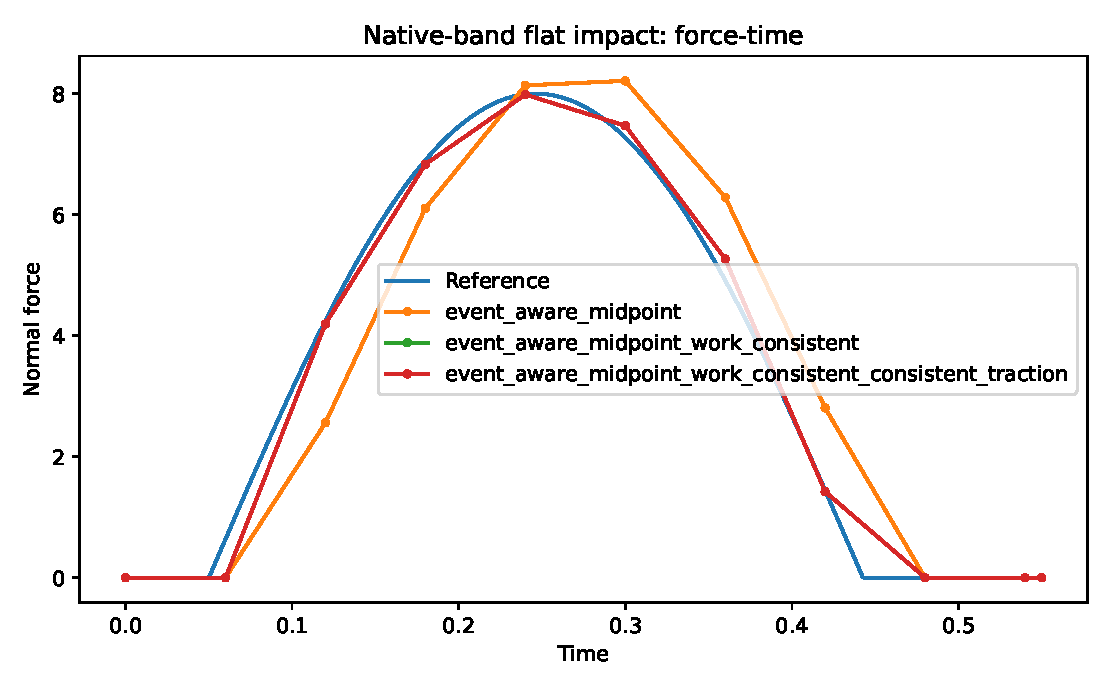
\includegraphics[width=0.82\linewidth]{native_band_force_time.pdf}
    \caption{Native-band flat 长时程 force-time 曲线。}
    \label{fig:native_force}
\end{figure}

\begin{figure}[H]
    \centering
    
\includegraphics[width=0.82\linewidth]{native_band_active_measure_time.pdf}
    \caption{Native-band flat 的 active-measure 演化。}
    \label{fig:native_active}
\end{figure}

\begin{figure}[H]
    \centering
    
\includegraphics[width=0.82\linewidth]{native_band_controller_statistics.pdf}
    \caption{Native-band flat 的 controller 统计量：predictor/corrector mismatch、work mismatch 与 force jump。}
    \label{fig:native_controller}
\end{figure}

\subsection{目前可以成立的结论与边界}
基于当前 Sprint 1 的代码、主表和图，本文认为以下结论已经可以成立：
\begin{enumerate}
    \item \textbf{SDF-native 主链已经打通。} 从 SDF 场构造、窄带 sparse traversal、local-normal correction，到 continuity-aware dynamics 与长时程 benchmark，主链是完整可运行的。
    \item \textbf{continuity 具有明确工程价值。} 它不仅是 active-set 的记录方式，更是统一动力学控制链中的关键数值机制，已经在不显著损伤主结果的前提下取得 traversal 成本收益。
    \item \textbf{时间一致性改进链是有效的。} 从 event-aware midpoint 到 impulse correction 再到 work consistency，关键长时程指标沿着清晰路线得到改进，并且这种改进在 flat 与 sphere 两类 benchmark 中都能观察到。
\end{enumerate}
同时也必须保持边界：native-band 动力学结果虽然已经足以支持“方向正确、机制有效”的结论，但还不足以宣称通用三维动力学精度问题已经完全解决；更一般三维复杂几何上的长时程证据链仍需继续补强。

\section{结论与展望}
Sprint 1 已经完成了从研究代码到投稿闭环基础设施的关键过渡。当前项目不仅具备一条完整的 SDF-native PFC 动力学求解主链，而且已经形成统一的长时程 benchmark、效率表、主图和导表脚本，使得论文中的核心结果可以由配置文件和实验脚本一键重现。现阶段最强的证据集中在 analytic flat、analytic sphere 和 native-band flat 三组 benchmark 上，它们共同支持如下阶段性结论：SDF-native 窄带求解可以在不依赖几何特调的前提下构成一条统一的动力学主链，continuity 与时间一致性是该主链中同时决定效率与精度的关键机制。

下一阶段的工作不应再简单堆叠新模块，而应沿两条线继续推进。第一条是 \textbf{通用性证据线}：补充偏心 flat、多 patch/disconnected 接触以及 controller 统计附表，进一步支撑“无特调通用框架”的论点。第二条是 \textbf{说服力补强线}：加入 reference comparison 与 sensitivity study，让审稿人能更清楚地看到 native-band 主链与高成本 reference 之间的关系，以及结果并非来自某组 magic parameter。换言之，Sprint 1 的完成并不意味着项目结束，而是意味着项目已经拥有一套足以支撑正式投稿打磨的可复现骨架。


\FloatBarrier
\clearpage
\appendix
\section{Sprint 2：通用性补充证据}
本附录补充 Sprint 2 引入的三组证据：偏心 flat benchmark、多 patch/disconnected 动态 benchmark 以及 controller statistics。其目的不是改变正文主结论，而是说明当前框架并不只对法向单 patch 场景有效，而是已经能够在偏心加载、多个活跃接触片以及显式 continuity/controller 统计层面给出可复现的结果。

\subsection{偏心 flat benchmark}
偏心 flat benchmark 的重点不在于把法向误差进一步做小，而在于证明当前 native-band 主链已经能够输出可比较的 torque 与 application-point 误差，从而把结论从标量法向力推广到 wrench 层面。表~\ref{tab:eccentric_flat} 给出了 analytic eccentric 与 native-band eccentric 两组结果。可以看到，解析模型上的 torque 指标已经较为稳定，而 native-band eccentric 仍然存在明显 torque/application-point 偏差，这一结果恰好说明：当前主瓶颈已经不再是接触建立时刻，而是更一般动态场景下的 traction consistency 与作用点一致性。

\begin{table}[H]
\caption{偏心 flat 基准中的 wrench 准确性}
\label{tab:eccentric_flat}
\resizebox{\linewidth}{!}{%
\begin{tabular}{lllllllll}
\toprule
Model & Scheme & Force error & Torque error & Peak torque error & Application point error & Impulse error & Energy drift & Release timing error \\
\midrule
analytic\_eccentric & event\_aware\_midpoint\_work\_consistent & 0.004126 & 0 & 0 & 0 & 0.007937 & 0.009755 & 0.002807 \\
native\_band\_eccentric & event\_aware\_midpoint\_work\_consistent & 0.134046 & 0.4375 & 0.4375 & 0.05 & 0.052509 & 0.036002 & 0.007301 \\
\bottomrule
\end{tabular}%
}
\end{table}


\subsection{多 patch / disconnected 动态 benchmark}
多 patch benchmark 用于检验 continuity/controller 在多个分离接触片场景中的稳定性。表~\ref{tab:multipatch_dynamic} 表明，在 analytic multipatch 场景下，当前 work-consistent 动力学器已经能够稳定跨越完整接触相位；而在 native-band multipatch 场景下，active component 数、predictor/corrector Jaccard 与 mismatch fraction 均已可量化地导出。这里最重要的不是误差绝对值已经最优，而是项目现在已经拥有了一个能够显式度量 split/merge 动态的实验接口。

\begin{table}[H]
\caption{多 patch 动态接触基准}
\label{tab:multipatch_dynamic}
\resizebox{\linewidth}{!}{%
\begin{tabular}{lllllllllll}
\toprule
Model & Scheme & Force error & Impulse error & Energy drift & Release timing error & Active component error & Mean active components & Max active components & Mean pred./corr. Jaccard & Mean mismatch fraction \\
\midrule
analytic\_multipatch & event\_aware\_midpoint\_work\_consistent & 0.004126 & 0.007937 & 0.009755 & 0.002807 & 0 & 1.714286 & 2 & -- & -- \\
native\_band\_multipatch & event\_aware\_midpoint\_work\_consistent & 0.249938 & 0.153464 & 0.186517 & 0.007301 & 0 & 2 & 2 & 0.717857 & 0.282143 \\
\bottomrule
\end{tabular}%
}
\end{table}


\subsection{Controller 统计量}
表~\ref{tab:controller_statistics} 总结了当前 controller 在偏心 flat 与 multipatch 场景中的主要统计量，包括 predictor/corrector Jaccard、mismatch fraction、work mismatch、各类 trigger 次数以及 candidate/recompute cells。它们说明 controller 已经不是黑箱逻辑，而是具有明确可报告行为的统一数值机制。对于后续论文打磨，这一组统计量还可以进一步转化为控制器行为图与附录消融表。

\begin{table}[H]
\caption{Controller 统计与通用性证据}
\label{tab:controller_statistics}
\resizebox{\linewidth}{!}{%
\begin{tabular}{lllllllllllll}
\toprule
Case & Mean pred./corr. Jaccard & Mean mismatch fraction & Max mismatch fraction & Mean work mismatch & Work mismatch triggers & Mismatch triggers & Force jump triggers & Measure jump triggers & Mean candidate cells & Mean recompute cells & Mean active components & Max active components \\
\midrule
native\_band\_eccentric & 0.717857 & 0.282143 & 1 & 0.028588 & 3 & 5 & 8 & 7 & 192 & 166 & 1 & 1 \\
native\_band\_multipatch & 0.717857 & 0.282143 & 1 & 0.005402 & 3 & 5 & 8 & 7 & 140 & 140 & 2 & 2 \\
\bottomrule
\end{tabular}%
}
\end{table}


\section{Sprint 3：参考解对比与敏感性分析}
Sprint 3 的目标是补强两类审稿人最关心的问题：第一，native-band 主链与 reference 之间的差距究竟有多大；第二，当前结果是否依赖某组 magic parameter。相应地，本附录给出 reference comparison 与 sensitivity suites 两套自动生成表。

\subsection{参考解对比}
表~\ref{tab:reference_comparison} 把当前默认工作流与三类 reference 放在同一个框架下比较：analytic flat 对 exact analytic 和 high-resolution same-scheme，analytic sphere 对 RK4 reference 和 high-resolution same-scheme，native-band flat 对 analytic flat exact 和 high-resolution native-band。该表支持一个重要判断：native-band flat 相对 high-resolution native-band 的误差明显小于其相对 analytic flat exact 的误差，这表明当前可见误差中既包含离散误差，也包含模型层差异；因此，后续工作既需要继续改善时间/空间离散，也需要更谨慎地区分“数值逼近误差”和“主链与解析模型之间的物理差异”。
\noindent\textit{For all native-band experiments in this paper, native-band now uses cell-centered volumetric sampling and cell-centered footprint support masking.}

\begin{table}[H]
\caption{参考解对比实验}
\label{tab:reference_comparison}
\resizebox{\linewidth}{!}{%
\begin{tabular}{llllllllllllll}
\toprule
Benchmark & Scheme & Reference & dt & Reference dt & State error & Peak force error & Impulse error & Release timing error & Rebound velocity error & Energy drift & Runtime (s) & Mean candidate cells & Mean recompute cells \\
\midrule
Analytic flat & + work consistency & Exact analytic & 0.04 & -- & 0.236853 & 6.591e-04 & 0.008664 & 7.424e-04 & 0.001131 & 0.001132 & 0.00556 & -- & -- \\
Analytic flat & + work consistency & High-res same scheme & 0.04 & 0.01 & 0.001548 & 0.002362 & 0.010156 & 8.073e-04 & 0.001117 & 0.001132 & 0.00556 & -- & -- \\
Analytic sphere & + work consistency & RK4 reference & 0.05 & 5.000e-04 & 4.986e-04 & 0.001686 & 0.001966 & 8.206e-04 & 7.514e-05 & -7.514e-05 & 0.031156 & -- & -- \\
Analytic sphere & + work consistency & High-res same scheme & 0.05 & 0.02 & 6.981e-04 & 0.001303 & 0.001971 & 7.258e-04 & 8.231e-05 & -7.514e-05 & 0.031156 & -- & -- \\
Native-band flat & + consistent traction reconstruction & Analytic flat exact & 0.06 & -- & 0.18338 & 0.198292 & 0.030332 & 0.075034 & 0.006008 & 0.006026 & 5.983681 & 122.727273 & 106.818182 \\
Native-band flat & + consistent traction reconstruction & High-res native-band & 0.06 & 0.02 & 0.003462 & 0.061817 & 0.035291 & 0.002051 & 0.003035 & 0.006026 & 5.983681 & 122.727273 & 106.818182 \\
\bottomrule
\end{tabular}%
}
\end{table}


\subsection{参数敏感性分析}
表~\ref{tab:sensitivity} 扫描了 grid spacing、band half width、$\eta$、work-mismatch tolerance、continuity 开关以及 consistent traction reconstruction 开关。当前结果说明：continuity 的主要收益体现在 candidate/recompute 数量下降，而不是把主误差“调小”；与此同时，$z$ 向分辨率、band 宽度与 $\eta$ 的变化会系统影响 peak force、impulse 和 energy drift。这些现象对论文写作有两个直接意义：一方面，它们足以支撑“结果并非来自单个特调参数”的论点；另一方面，也明确指出 native-band 主链后续最值得继续优化的敏感方向仍是局部窄带离散与 traction consistency。

\begin{table}[H]
\caption{敏感性分析}
\label{tab:sensitivity}
\resizebox{\linewidth}{!}{%
\begin{tabular}{llrllllllll}
\toprule
Parameter & Value & Baseline & Peak force error & Impulse error & Energy drift & Release timing error & Runtime (s) & Mean candidate cells & Mean recompute cells & Mean substeps \\
\midrule
baseline & default & True & 0.198292 & 0.030332 & 0.006026 & 0.075034 & 6.812135 & 122.727273 & 106.818182 & 1 \\
grid\_spacing\_z & 0.0200 & False & 0.222404 & 0.035463 & -0.016715 & 0.072853 & 3.518825 & 77.272727 & 77.272727 & 1 \\
grid\_spacing\_z & 0.0100 & False & 0.198292 & 0.030332 & 0.006026 & 0.075034 & 6.778946 & 122.727273 & 106.818182 & 1 \\
grid\_spacing\_z & 0.0050 & False & 0.206797 & 0.035773 & 0.012443 & 0.074066 & 11.34986 & 172.727273 & 152.272727 & 1 \\
band\_half\_width & 8.00 & False & 0.17712 & 0.04189 & 0.009759 & 0.070852 & 5.276463 & 106.818182 & 106.818182 & 1 \\
band\_half\_width & 12.00 & False & 0.198292 & 0.030332 & 0.006026 & 0.075034 & 6.927674 & 122.727273 & 106.818182 & 1 \\
band\_half\_width & 16.00 & False & 0.198292 & 0.030332 & 0.006026 & 0.075034 & 6.802415 & 122.727273 & 106.818182 & 1 \\
eta & 6.00 & False & 0.176774 & 0.038426 & 0.003712 & 0.07341 & 6.484379 & 122.727273 & 106.818182 & 1 \\
eta & 8.00 & False & 0.198292 & 0.030332 & 0.006026 & 0.075034 & 6.585999 & 122.727273 & 106.818182 & 1 \\
eta & 10.00 & False & 0.214222 & 0.020924 & 0.003524 & 0.07314 & 6.676618 & 122.727273 & 106.818182 & 1 \\
work\_mismatch\_relative\_tol & 0.020 & False & 0.198292 & 0.030332 & 0.006026 & 0.075034 & 6.890314 & 122.727273 & 106.818182 & 1 \\
work\_mismatch\_relative\_tol & 0.050 & False & 0.198292 & 0.030332 & 0.006026 & 0.075034 & 6.655358 & 122.727273 & 106.818182 & 1 \\
work\_mismatch\_relative\_tol & 0.100 & False & 0.198292 & 0.030332 & 0.006026 & 0.075034 & 6.587981 & 122.727273 & 106.818182 & 1 \\
continuity\_enabled & False & False & 0.198292 & 0.030332 & 0.006026 & 0.075034 & 7.067634 & 286.363636 & 286.363636 & 1 \\
continuity\_enabled & True & False & 0.198292 & 0.030332 & 0.006026 & 0.075034 & 6.9068 & 122.727273 & 106.818182 & 1 \\
consistent\_traction\_reconstruction & False & False & 0.198292 & 0.030332 & 0.006026 & 0.075034 & 7.168637 & 122.727273 & 106.818182 & 1 \\
consistent\_traction\_reconstruction & True & False & 0.198292 & 0.030332 & 0.006026 & 0.075034 & 7.30704 & 122.727273 & 106.818182 & 1 \\
\bottomrule
\end{tabular}%
}
\end{table}


\section{附录小结}
截至当前版本，本文已经在正文主表之外补齐了三类附录证据：其一，偏心 flat 与 multipatch benchmark 将结论从法向力扩展到 wrench 与多接触片动态；其二，controller statistics 使 continuity/controller 机制具备可解释的行为统计；其三，reference comparison 与 sensitivity suites 为 native-band 主链提供了更完整的说服力边界。它们共同说明：当前项目已经不仅能写出一条主结果线，也已经逐步具备高水平论文所要求的附录证据结构。

\end{document}
